%!TEX root = ../dissertation.tex

\chapter{Introduction}
\label{chapter:introduction}

The Medical Imaging Multimodality Breast Cancer Diagnosis is a topic of great interest, it has been the subject of intensive research in the world of medicine. However the developments in terms of innovation in the computational world are still scarce. The Interface herein proposer deals with the processing and analysis of images. Indeed, this topic has a wide spectrum of applications raging from video surveillance based systems to medical applications.

In the proposed work, i.e., the analysis mammography using multi-modality images, several issues must be considered. First each image modality has its own image features. Which must be included in the interface. Second, for each image modality several and distinct image feature must be considered.

Masses and calcifications can be accurately diagnosed from cytological features \cite{Mangasarian95breastcancer} of the cells that constitute them. However, the diagnostic accuracy depends on the training, experience, and many indefinite factors of interpretation of the medical expert in cytological evaluation.

There were, in fact, some developments in the past facing the Computer-Based classification system \cite{Bennett92robustlinear, Mangasarian98multisurfacemethod} that assists in the diagnosis of breast cells based on visual assessment of characteristics of the cells. A set of cytologic features \cite{Wolberg90}, previously evaluated visually, are now replaced by digital ones, evaluated by image analysis. In this project, the interface will be used by several experts in the field, to collect the ground truth, for Mammograms, \gls{MRI} and Ultrasounds images. Those mammography experts annotations will be a crucial step towards the performance evaluation of Machine Learning (ML) Based-Algorithms.

Doctors are accountable for decisions they make on behalf of their patients. Likewise, computer interface developers and engineers must assume accountability for limitations, assumptions and other unplanned deficiencies that impact on the integrity, validity, quantity and timeliness of data made accessible through their interfaces.

Art and science \cite{cukier2011artist} applied to the user interface filed of clinical care are based on an unusual combination of non-judgement trust and exasperating mistrust \cite{kahn1998keep}. Two major obstacles to good clinicians-patient communication are differences of language and culture \cite{sielhorst2008advanced}. Doctors and clinicians require that theirs patients keep no secrets or else an opportunity to reach the right diagnosis or select the proper therapy may be lost. At the same time, doctors and clinicians are taught to question everything they hear from both colleagues and patients. It is deeply ingrained in medical training to make no important decisions based on information supplied solely by others. The highly trained mistrust explains why many times patients complained that a dozen different people asked the same question. A deeply ingrained aversion to secrets and lies greatly characterise a clinician’s attitude toward a computer interface where the responsibility of interface developers address and incorporate the concept of visual accountability extending well beyond medical user interfaces.

\clearpage

% Commands to include a figure:
\begin{figure}[!hbt]
\centering
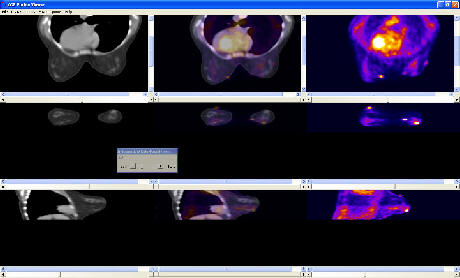
\includegraphics[width=15cm]{images/multimodalbreastimage}~\\
\caption{\label{fig:screenshot}A screenshot of a fused data set.
}
\end{figure}

The growing interest in multimodal interface development is inspired in large part by goals of supporting more flexible, transparent, efficient and powerfully expressive means of human-computer interaction than in the past. Multimodal interfaces are expected to support a wider range of diverse applications, be usable by a broader spectrum of the average population, and function more reliably under realistic and challenging usage conditions.

Computer-aided  diagnosis  often  implies  processing large and high dimensional datasets, for instance, high-resolution volumes containing millions of voxels.

Visualisation and analysis of such data can be very time demanding for physicians but also very computationally expensive for machines assisting diagnosis tasks. Fortunately, in many cases the relevant information for an application can be represented in lower dimensional spaces. If appropriately  chosen and designed, dimensionality reduction methods will not only decrease the processing time but also facilitate any posterior analysis. Therefore, they can be of great use to a variety of \gls{CAD}  applications, ranging  from  general problems such as classification and visualisation, to more specific ones like multi-modal registration or motion compensation.

Dimensionality reduction in \gls{CAD} has relied mainly on linear methods and linear  methods  are  however not suitable for handling non-linear complex relationships among the data samples. Non-linear approaches based on manifold learning are a good alternative for dimensionality reduction in such cases.

Medical Imaging Multimodality Breast Cancer Diagnosis User Interface (MIMBCD-UI)  registration  consists  in  finding  a map between images of the same scene acquired with different imaging modalities. The standard approach to multi-modal registration is to use sophisticated similarity metrics such as mutual information to compare the images.
